\let\negmedspace\undefined
\let\negthickspace\undefined
\documentclass[journal]{IEEEtran}
\usepackage[a5paper, margin=10mm, onecolumn]{geometry}
%\usepackage{lmodern} % Ensure lmodern is loaded for pdflatex
\usepackage{tfrupee} % Include tfrupee package

\setlength{\headheight}{1cm} % Set the height of the header box
\setlength{\headsep}{0mm}     % Set the distance between the header box and the top of the text

\usepackage{gvv-book}
\usepackage{gvv}
\usepackage{cite}
\usepackage{amsmath,amssymb,amsfonts,amsthm}
\usepackage{algorithmic}
\usepackage{graphicx}
\usepackage{textcomp}
\usepackage{xcolor}
\usepackage{txfonts}
\usepackage{listings}
\usepackage{enumitem}
\usepackage{mathtools}
\usepackage{gensymb}
\usepackage{comment}
\usepackage[breaklinks=true]{hyperref}
\usepackage{tkz-euclide} 
\usepackage{listings}
% \usepackage{gvv}                                        
\def\inputGnumericTable{}                                 
\usepackage[latin1]{inputenc}                                
\usepackage{color}                                            
\usepackage{array}                                            
\usepackage{longtable}                                       
\usepackage{calc}                                             
\usepackage{multirow}                                         
\usepackage{hhline}                                           
\usepackage{ifthen}                                           
\usepackage{lscape}
\begin{document}

\bibliographystyle{IEEEtran}
\vspace{3cm}

\title{
3 - Constructions \\
\large EE1030:Matrix Theory
}
\author{Gajjarapu Satyanarayana\\AI24BTECH11009
}
% \maketitle
% \newpage
% \bigskip
{\let\newpage\relax\maketitle}

\renewcommand{\thefigure}{\theenumi}
\renewcommand{\thetable}{\theenumi}



\numberwithin{equation}{enumi}
\numberwithin{figure}{enumi}
\renewcommand{\thetable}{\theenumi}


\textbf{Question}:3.2.21\\
Construct and give justification:\\
A right triangle when one side is 3.5 cm and sum other side and the hypotenuse is 5.5 cm.
\\
\textbf{Solution:}
\renewcommand{\tablename}{Table 3.2.21.1}
\begin{table}[h!]
  \centering
  \begin{tabular}[12pt]{ |c| c|}
    \hline
    \textbf{Variables} & \textbf{Description}\\ 
    \hline
    $\textbf{V}_1, \vec{u}_1, f_1$ & Parameters of the parabola $y^2 = 4x$ \\
    \hline
     $\textbf{V}_2, \vec{u}_2, f_2$ & Parameters of the circle $4x^2 + 4xy^2 = 9$ \\
    \hline
    $\vec{x}^\intercal\brak{\textbf{V}_1 + \mu\textbf{V}_2}\vec{x} + 2\brak{\vec{u}_1 + \mu\vec{u}_2}^\intercal\vec{x} + \brak{f_1 + \mu f_2}$ & Intersection of two conics \\
    \hline
    \end{tabular}


  \caption{Variables and its values}
\end{table}
\\
Consider the right angle at $\vec{B}$, so that $\angle B$ = 90\degree, $\cos{\brak{\angle B}} = 0$, $\sin{\brak{\angle B}} = 1$\\
In $\triangle ABC$, if $\vec{B}$ is considered as origin then the coordinates are represented by
 \begin{align}
 \vec{A} & = c\myvec{\cos{\brak{\angle B}} \\ \sin{\brak{\angle B}}} \\
 \vec{A} & = \myvec{0 \\ c} \\
 \vec{B} & = \myvec{0 \\ 0} \\
 \vec{C} & = \myvec{a \\ 0}
 \end{align}
Using the formula to find c,
\begin{align}
c & = \frac{k^2 - a^2}{2\brak{k - a\cos{\brak{\angle B}}}} \\
c & = \frac{\frac{121}{4} - \frac{49}{4}}{2\brak{\frac{11}{2} - 0}} \\
c & = \frac{18}{11}
\end{align}
Therefore,
\begin{align}
    \vec{A} & = \myvec{0 \\ \frac{18}{11}} \\
    \vec{B} & = \myvec{0 \\ 0} \\
    \vec{C} & = \myvec{\frac{7}{2} \\ 0}
\end{align}
\begin{figure}[h!]
   \centering
   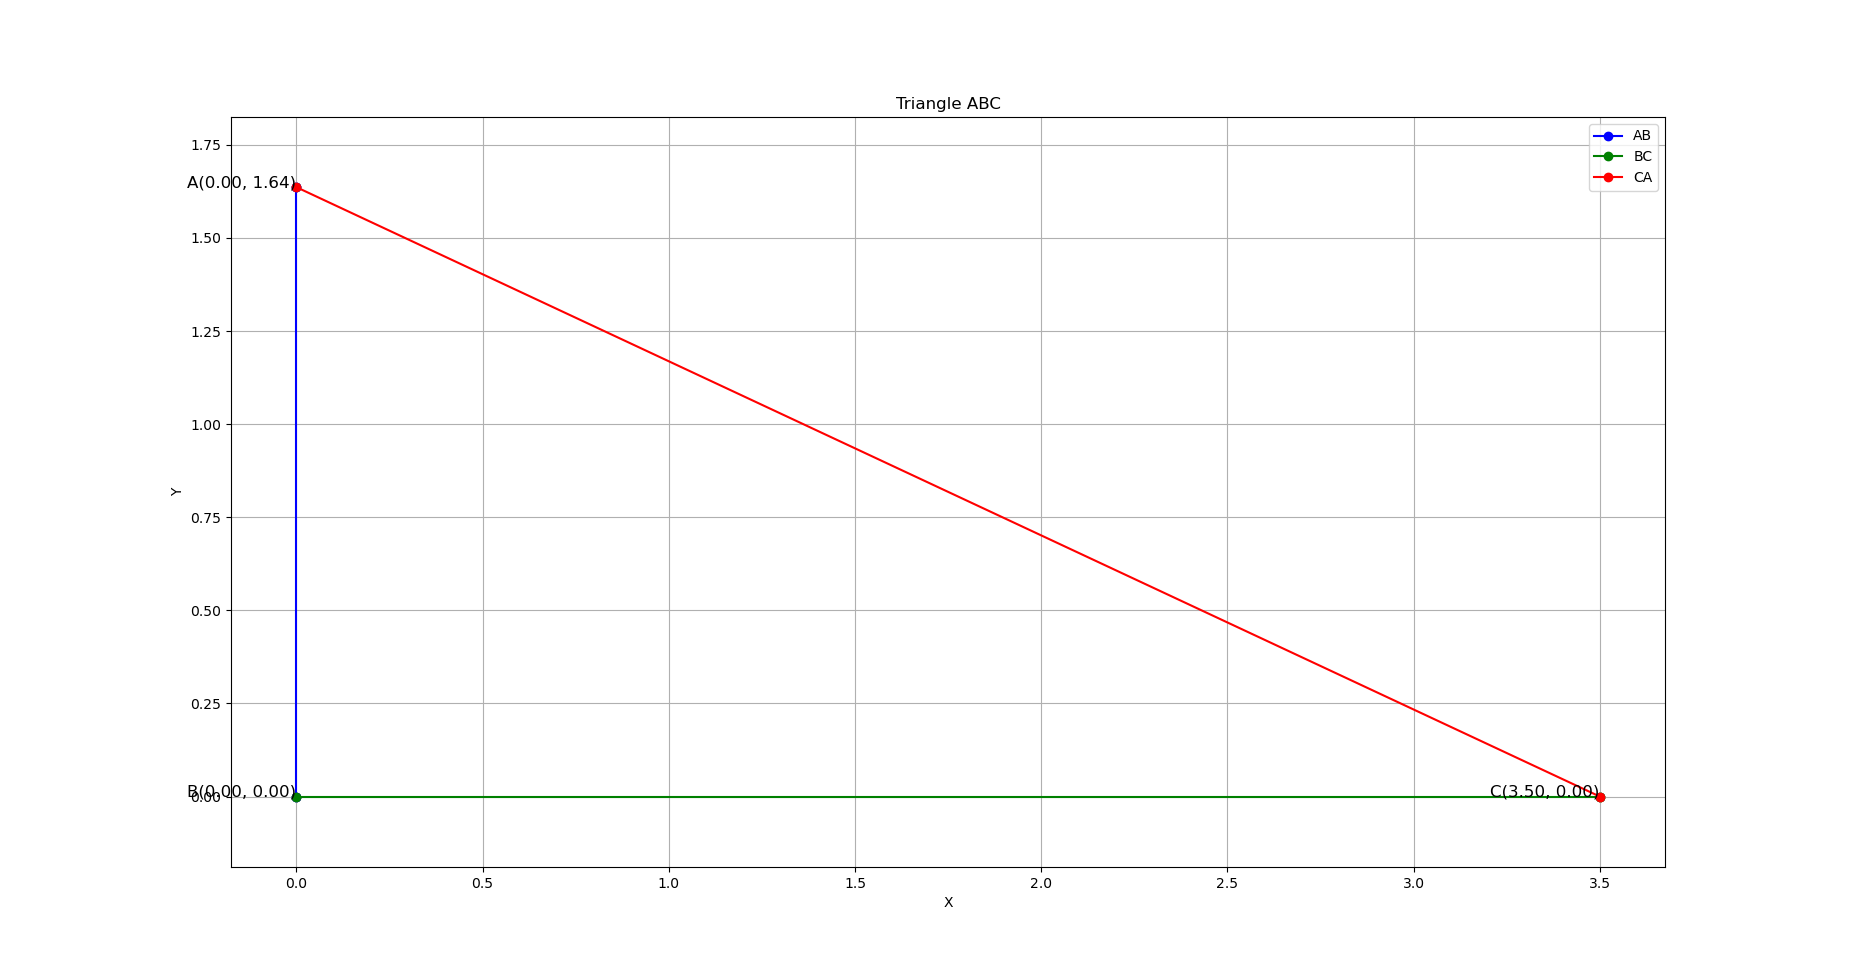
\includegraphics[width=0.7\linewidth]{figs/triangle.png}
	\caption{Triangle $ABC$}
   \end{figure}
\end{document}

